\documentclass[a4paper,11pt]{article}

\usepackage[utf8]{inputenc}
\title{ARC2 -- TP 6}
\author{Prune Forget, Léo Noël-Baron \& Thierry Sampaio}
\date{09/03/2016}

\usepackage{a4wide}
\usepackage{textcomp}
\usepackage[utf8]{inputenc}
\usepackage[T1]{fontenc}
\usepackage[francais]{babel}

\usepackage{graphicx}
\usepackage[usenames,dvipsnames]{color}

\usepackage{hyperref} \urlstyle{sf}
\hypersetup{
  colorlinks=true,
  urlcolor=BlueViolet,
  citecolor=BlueViolet,
  linkcolor=BlueViolet,
}
\DeclareUrlCommand\email{\urlstyle{sf}}

\newenvironment{keywords}
  {\description\item[\bsc{Mots-clés}]~$\cdot$~ }
  {\enddescription}
\newenvironment{remarque}
  {\description\item[\bsc{Remarque} ---]\sl}
  {\enddescription}
\renewcommand{\thefootnote}{\arabic{footnote}}

\usepackage{listings}
\lstset{
  language=C,
  basicstyle=\ttfamily,
  keywordstyle=\color{OliveGreen},
  stringstyle=\color{Bittersweet},
  showstringspaces=false,
  commentstyle=\color{Gray},
  numbers=left,
  numberstyle=\ttfamily\color{Gray},
  frame=l,
  columns=fullflexible,
  rulecolor=\color{Gray},
  tabsize=4,
  extendedchars=true,
  literate=
	{É}{{\'E}}1 {è}{{\`e}}1 {à}{{\`a}}1 {È}{{\`E}}1 {À}{{\`A}}1 {ê}{{\^e}}1 {â}{{\^a}}1 {î}{{\^\i}}1 {ô}{{\^o}}1
	{Ê}{{\^E}}1 {Â}{{\^A}}1 {Î}{{\^I}}1 {Ô}{{\^O}}1 {Û}{{\^U}}1 {ë}{{\"e}}1 {ï}{{\"\i}}1 {ü}{{\"u}}1 {Ë}{{\"E}}1
	{Ï}{{\"I}}1 {Ü}{{\"U}}1 {û}{{\^u}}1 {ç}{{\c c}}1 {Ç}{{\c C}}1 {æ}{{\ae}}1 {Æ}{{\AE}}1 {œ}{{\oe}}1 {Œ}{{\OE}}1
	{é}{{\'e}}1,
}
\lstMakeShortInline{|}

\parskip=0.3\baselineskip
\sloppy

\makeatletter
  \let\runtitle\@title
  \let\runauthor\@author
\makeatother

\usepackage{fancyhdr}
\pagestyle{fancy}
\fancyhead{}
\lhead{\runtitle}
\rhead{\runauthor}
\setlength{\headheight}{13.6pt}


\begin{document}

\maketitle

\subsection*{Mémoire de 256 bits}

On crée tout d'abord un composant mémoire en suivant les indications de l'énoncé. On choisit de le brancher à l'adresse 2048, ce qui permet de réaliser les signaux de lecture et d'écriture de ce composant en conjuguant \verb?Lec? et \verb?Ecr? avec le bit 11 du registre \verb?MA?. L'adresse d'un mot de 32 bits se lit alors sur \verb?MA[4..2]?, ce qui donne les branchements en Figure \ref{membits}.

\begin{figure}[h]\center
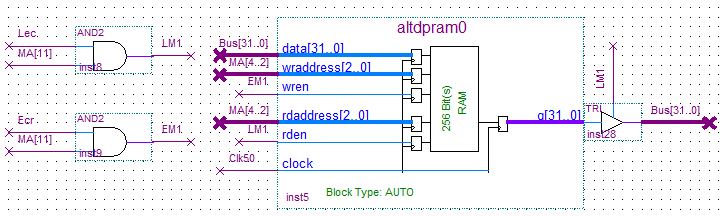
\includegraphics[scale=0.7]{tp6-1.PNG}
\caption{Mémoire de 256 bits}
\label{membits}
\end{figure}

\subsection*{Mémoire de 16 mots}

On crée maintenant un composant mémoire différent. On choisit de le brancher à l'adresse 4096, ce qui permet de réaliser les signaux de lecture et d'écriture avec \verb?Lec?, \verb?Ecr? et le bit 12 de \verb?MA?. Comme le composant contient 16 mots de 32 bits, l'adressage doit se faire avec les 3 bits \verb?MA[5..2]?, ce qui donne les branchements en Figure \ref{memwords}.

\begin{figure}[h]\center
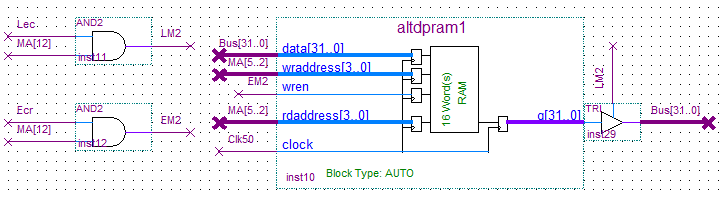
\includegraphics[scale=0.7]{tp6-2.PNG}
\caption{Mémoire de 16 mots}
\label{memwords}
\end{figure}

Voici le programme utilisé pour tester (avec succès) ces deux composants :
\begin{lstlisting}[language=Lisp]
      ; Stockage de 244 et 12 dans les deux mémoires
      addi r6,r0,244
      stw  r6,2048(r0)
      addi r6,r0,12
      stw  r6,4100(r0)
      ; Récupération et sommation des valeurs
      ldw  r7,2048(r0)
      ldw  r8,4100(r0)
      add  r7,r7,r8
      stw  r7,1024(r0)
.end
\end{lstlisting}

\end{document}
